\section{Fundamentos teóricos de las emociones}

El estudio de las emociones ha sido abordado desde múltiples disciplinas como la psicología, la neurociencia, la filosofía y las ciencias cognitivas. En el ámbito de la Inteligencia Artificial y la computación afectiva, las teorías psicológicas de las emociones constituyen la base conceptual para el desarrollo de modelos computacionales capaces de representar estados emocionales y su influencia en el comportamiento de agentes inteligentes.

En términos generales, las emociones pueden interpretarse como mecanismos que influyen sobre cómo un individuo percibe situaciones, prioriza información y toma decisiones frente al entorno. Diversos estudios han demostrado que las emociones no actúan únicamente como reacciones impulsivas, sino que participan activamente en mecanismos de razonamiento y adaptación al entorno \cite{alfonso2021affect}.

\subsection{Teorías clásicas de las emociones}

Existen diferentes enfoques para describir y clasificar las emociones humanas. Algunas teorías consideran las emociones como categorías discretas, mientras que otras las representan mediante dimensiones continuas.

Uno de los enfoques más conocidos es el modelo de emociones básicas de Ekman \cite{ekman1992argument}, que propone un conjunto reducido de emociones universales presentes en todas las culturas humanas, entre ellas alegría, tristeza, miedo, ira, sorpresa y asco. Estas emociones básicas se consideran biológicamente innatas y asociadas a expresiones faciales universales.

Otro modelo ampliamente utilizado es la rueda de emociones de Plutchik \cite{plutchik1980general}, que organiza las emociones en pares opuestos y establece distintos niveles de intensidad emocional. Este modelo introduce además relaciones de combinación entre emociones primarias, permitiendo representar emociones más complejas.

Desde una perspectiva dimensional, Russell propuso el modelo circumplejo de emociones \cite{russell1980circumplex}, donde los estados emocionales se representan mediante dimensiones continuas relacionadas principalmente con valencia emocional y nivel de activación. Este enfoque resulta especialmente útil en computación afectiva debido a su facilidad para representar transiciones emocionales dinámicas.

\subsection{Modelo PAD}

Uno de los modelos dimensionales más utilizados en agentes afectivos es el modelo PAD (\textit{Pleasure-Arousal-Dominance}). Este modelo representa cada estado emocional mediante tres dimensiones continuas \cite{mehrabian1974approach}:

\begin{itemize}
    \item \textbf{Pleasure}: grado de agrado o desagrado emocional.
    \item \textbf{Arousal}: nivel de activación o excitación.
    \item \textbf{Dominance}: sensación de control o sumisión.
\end{itemize}

De forma general, un estado emocional puede representarse mediante el vector:

\begin{equation}
    \vec{Mood} = (P, A, D)
\end{equation}

donde $P$ representa la valencia emocional, $A$ el nivel de activación y $D$ la sensación de dominancia.

\begin{figure}[H]
    \centering
    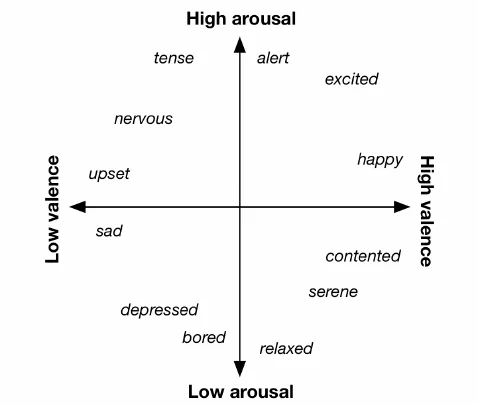
\includegraphics[width=0.60\textwidth]{figures/PAD.png}
    \caption{Proyección bidimensional (Valencia-Arousal) relacionada con modelos dimensionales. El modelo PAD completo incorpora una tercera dimensión (Dominancia) \cite{article}.}
    \label{fig:pad_model}
\end{figure}

Este tipo de representación permite modelar emociones de manera continua y facilita la simulación de cambios emocionales graduales en agentes inteligentes. Además, el modelo PAD ha sido ampliamente utilizado en sistemas de interacción humano-computador, personajes virtuales y agentes conversacionales debido a su simplicidad matemática y flexibilidad computacional.

En muchos modelos afectivos, las emociones evolucionan dinámicamente en función de estímulos internos y externos. Una formulación simplificada de actualización emocional puede expresarse como:

\begin{equation}
Mood_{t+1} = \beta \cdot Mood_t + \alpha \cdot Emotion
\end{equation}

donde $\beta$ representa la persistencia del estado emocional previo y $\alpha$ la influencia del nuevo estímulo emocional sobre el agente.

\subsection{Modelo OCC}

Uno de los modelos más influyentes dentro de la computación afectiva es el modelo OCC (\textit{Ortony, Clore and Collins}), propuesto originalmente para describir la estructura cognitiva de las emociones. Este modelo clasifica las emociones en función de la evaluación cognitiva (\textit{appraisal}) realizada por un individuo sobre eventos, acciones y objetos \cite{occ2009revisited}.

La revisión propuesta por Steunebrink et al. busca resolver algunas ambigüedades presentes en la formulación original de OCC, especialmente en relación con la representación lógica y formal de determinadas emociones complejas \cite{occ2009revisited}.

El modelo OCC organiza las emociones en tres grandes categorías principales:

\begin{itemize}
    \item Emociones relacionadas con las consecuencias de eventos.
    \item Emociones relacionadas con las acciones de agentes.
    \item Emociones relacionadas con aspectos de objetos.
\end{itemize}

A partir de esta estructura, OCC relaciona determinadas evaluaciones cognitivas con emociones concretas. Por ejemplo, el miedo aparece cuando el agente anticipa un evento negativo futuro, mientras que la gratitud surge cuando otro agente realiza una acción considerada beneficiosa.

A pesar de seguir siendo una referencia clásica dentro de la computación afectiva, distintos autores han señalado ciertas ambigüedades en la formalización lógica original de OCC. Steunebrink et al. \cite{occ2009revisited} destacan que algunas categorías emocionales presentan relaciones poco precisas entre eventos, acciones y objetos, dificultando su implementación computacional exacta. Como respuesta, proponen una reinterpretación basada en herencia lógica que clarifica la estructura jerárquica de las emociones y facilita su integración en arquitecturas de agentes inteligentes.

\begin{table}[H]
\centering
\caption{Ejemplos de emociones en el modelo OCC}
\begin{tabular}{|l|l|}
\hline
\textbf{Evaluación cognitiva} & \textbf{Emoción asociada} \\ \hline
Evento deseable & Alegría \\ \hline
Evento indeseable & Malestar \\ \hline
Prospecto deseable & Esperanza \\ \hline
Prospecto indeseable & Miedo \\ \hline
Acción propia aprobable & Orgullo \\ \hline
Acción ajena reprobable & Reproche \\ \hline
Acción ajena beneficiosa & Gratitud \\ \hline
\end{tabular}
\label{tab:occ}
\end{table}

\subsection{Emociones y razonamiento}

Diversos trabajos en neurociencia y psicología cognitiva han mostrado que las emociones influyen directamente sobre procesos racionales y deliberativos. Las emociones afectan a la memoria, la atención selectiva, la evaluación de riesgos y la priorización de objetivos \cite{alfonso2021affect}.

En el contexto de agentes inteligentes, esta relación entre emoción y cognición resulta especialmente relevante en entornos dinámicos e inciertos, donde los agentes deben actuar con recursos limitados y bajo condiciones cambiantes. Incorporar emociones permite reducir espacios de búsqueda, priorizar acciones relevantes y adaptar el comportamiento social de los agentes.